\chapter{مقدمه}
\label{chap:1}


\section*{چکیده}

در این فصل، مفاهیم پایه هر دو حوزه امنیت لایه فیزیکی\LTRfootnote{Physical-layer security (PLS)} (\lr{PLS}) و توزیع کلید کوانتومی\LTRfootnote{Quantum key distribution (QKD)} (\lr{QKD}) معرفی می‌شوند. فصل با بررسی نقش \lr{PLS} آغاز شده و با مروری کوتاه بر سیستم‌های رمزنگاری متداول مبتنی بر کلید ادامه می‌یابد. سپس مفهوم امنیت نظریه-اطلاعاتی\LTRfootnote{Information-theoretic security} معرفی شده و شرط محرمانگی کامل\LTRfootnote{Perfect secrecy condition} تشریح می‌گردد. امنیت محاسباتی\LTRfootnote{Computational security} به‌عنوان مورد خاصی از امنیت نظریه-اطلاعاتی توصیف می‌شود که در آن چندین مورد تعدیل\LTRfootnote{Relaxation} معرفی شده است. در ادامه، مفاهیم محرمانگی قوی و ضعیف ارائه می‌شوند. علاوه بر این، مدل کانال شنود تخریب‌شده\LTRfootnote{Degraded wiretap channel} که توسط واینر\LTRfootnote{Wyner} معرفی شده، توصیف گردیده و کدهای کانال شنود متناظر تعریف می‌شوند. سپس، کانال پخش با پیام‌های محرمانه\LTRfootnote{Broadcast channel with confidential messages} که توسط سیزار\LTRfootnote{Csiszár} و کورنر\LTRfootnote{Körner} معرفی شده است، به همراه کد تصادفی\LTRfootnote{Stochastic code} مربوطه شرح داده می‌شود. آخرین موضوع در بخش \lr{PLS} به پروتکل توافق کلید مخفی اختصاص یافته است. بخش \lr{QKD} ابتدا نحوه شکستن پروتکل \lr{RSA} را به کمک الگوریتم تجزیه شور\LTRfootnote{Shor’s factorization algorithm} توصیف کرده و در ادامه توصیف کوتاهی از مبانی طرح‌های \lr{QKD} با متغیر گسسته\LTRfootnote{Discrete variable (DV)} (\lr{DV}) و متغیر پیوسته\LTRfootnote{Continuous variable (CV)} (\lr{CV}) ارائه می‌دهد. محدودیت‌های کلیدی طرح‌های \lr{DV-QKD} شناسایی شده و پروتکل‌های مختلف \lr{QKD} در سه دسته کلی قرار می‌گیرند: \lr{QKD} وابسته به دستگاه، \lr{QKD} مستقل از دستگاه منبع و \lr{QKD} مستقل از دستگاه اندازه‌گیری\LTRfootnote{Measurement device-independent (MDI)} (\lr{MDI}). علاوه بر این، تعریف کسر محرمانگی\LTRfootnote{Secrecy fraction} برای پروتکل‌های \lr{QKD} ارائه شده و به‌دنبال آن شرح کوتاهی از حملات انفرادی (غیرهمدوس) و دسته‌جمعی، و توضیحی درباره نحوه محاسبه کسر محرمانگی متناظر آورده شده است. در بخش سازمان‌دهی کتاب، توصیف دقیقی از محتوای فصل‌ها ارائه می‌گردد.

\section{مبانی امنیت لایه فیزیکی}
\label{sec:1-1}
رمزنگاری کلید عمومی دارای چندین نقص جدی است، از جمله: پیاده‌سازی آن در دستگاه‌هایی با محدودیت حافظه و پردازش پایین دشوار است، اینترنت به‌طور فزاینده‌ای در حال متحرک شدن است، طرح‌های امنیتی بر پایه فرضیات اثبات‌نشده‌ای از دشواری\LTRfootnote{Intractability} توابع خاص بنا شده‌اند، و فرضِ محدود بودن منابع محاسباتی ایو\LTRfootnote{Eve} در بسیاری از موارد نادرست است. مدل مرجع اتصال متقابل سیستم‌های باز\LTRfootnote{Open system interconnection (OSI)} (\lr{OSI}) هفت لایه را تعریف می‌کند. با این حال، در شکل \ref{fig:1-1} تنها پنج لایه مرتبط با مسائل امنیتی ارائه شده است. مدل اصلی \lr{OSI} حتی مسائل امنیتی را به‌هیچ‌وجه مشخص نمی‌کند. مسائل امنیتی در استاندارد \lr{X.800} (معماری امنیتی برای \lr{OSI}) مورد توجه قرار گرفته‌اند \cite{1-1}. با این حال، نه امنیت لایه فیزیکی (\lr{PLS}) \cite{1-2, 1-3, 1-4, 1-5, 1-6} و نه توزیع کلید کوانتومی (\lr{QKD}) \cite{1-7, 1-8, 1-9, 1-10, 1-11} در این استاندارد مورد بحث قرار نگرفته‌اند. با این وجود، سرویس‌های مشخص‌شده در این پنج لایه را می‌توان با به‌کارگیری \lr{PLS} و \lr{QKD} به‌طور قابل‌توجهی بهبود بخشید. طرح‌های \lr{PLS} و \lr{QKD} می‌توانند به‌صورت مستقل نیز عمل کنند.

\begin{figure}[ht]
	\centering
	 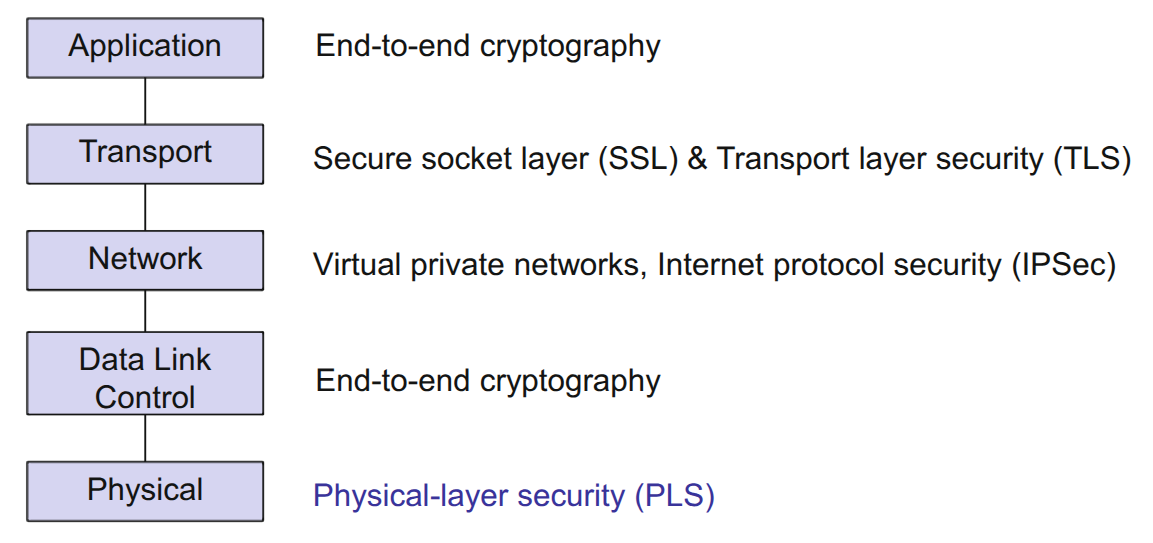
\includegraphics[width=0.8\textwidth]{chapters/figs/fig-1-1}
	\caption{مکانیزم‌های امنیتی در لایه‌های مختلف مدل \lr{OSI}. تنها لایه‌های مرتبط با امنیت نشان داده شده‌اند.}
	\label{fig:1-1}
\end{figure}

\begin{figure}[ht]
	\centering
	 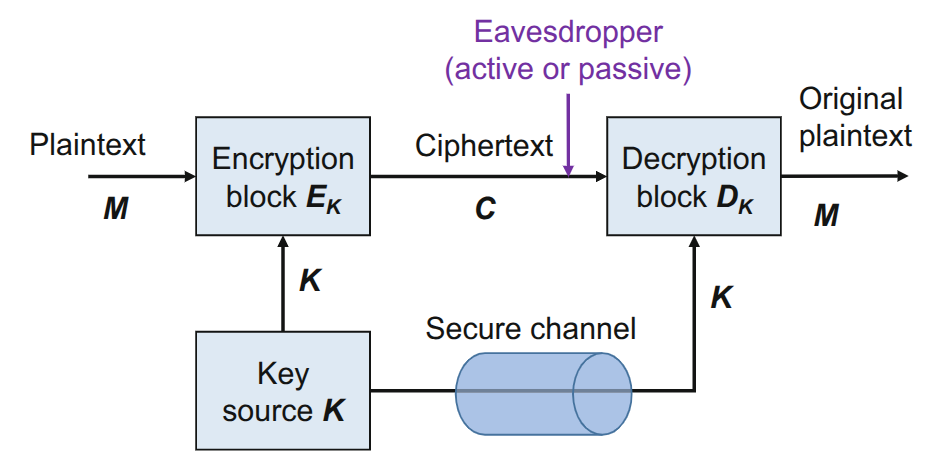
\includegraphics[width=0.8\textwidth]{chapters/figs/fig-1-2}
	\caption{طرح رمزنگاری پایه مبتنی بر کلید.}
	\label{fig:1-2}
\end{figure}

\begin{figure}[ht]
	\centering
	 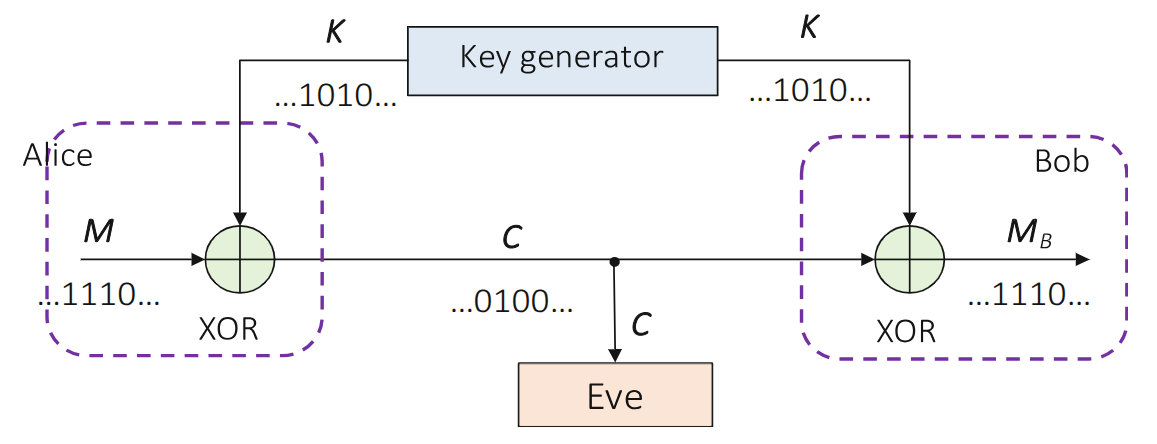
\includegraphics[width=0.8\textwidth]{chapters/figs/fig-1-3}
	\caption{طرح رمزگذاری پد یک‌بار مصرف.}
	\label{fig:1-3}
\end{figure}

سیستم رمزنگاری پایه مبتنی بر کلید \cite{1-12, 1-13, 1-14, 1-15, 1-16, 1-17, 1-18, 1-19, 1-20, 1-21, 1-22} در شکل \ref{fig:1-2} ارائه شده است. منبع، پیام (متن‌آشکار\LTRfootnote{Plaintext}) $M$ را به سمت بلوک رمزگذاری ارسال می‌کند که این بلوک با کمک کلید $K$ دریافت شده از منبع کلید، رمزنگاشت (متن‌رمز\LTRfootnote{Ciphertext}) $C$ را تولید می‌کند. در سمت گیرنده، رمزنگاشت ارسال شده از طریق یک کانال ناامن، توسط الگوریتم رمزگشایی به همراه کلید $K$ که از طریق کانال امن دریافت شده است، پردازش می‌شود که متن‌آشکار اصلی را برای تحویل به کاربر احرازهویت‌شده بازسازی می‌کند. فرآیند رمزگذاری را می‌توان به‌صورت ریاضی به‌صورت $E_K(M) = C$ توصیف کرد، در حالی که فرآیند رمزگشایی با $D_K(C) = M$ بیان می‌شود. ترکیب توابع رمزگشایی و رمزگذاری منجر به نگاشت همانی 	$D_K(E_K(M)) = M$ می‌گردد.
منبع کلید معمولاً کلید را به‌صورت تصادفی از فضای کلید\LTRfootnote{Keyspace} (محدوده مقادیر ممکن برای کلید) تولید می‌کند.


الگوریتم‌های مبتنی بر کلید را می‌توان به دو دسته کلی تقسیم کرد:
\begin{itemize}
	\item \textbf{الگوریتم‌های متقارن\LTRfootnote{Symmetric algorithms}:} که در آن‌ها کلید رمزگشایی را می‌توان از کلید رمزگذاری مشتق کرد و بالعکس. متناوباً، می‌توان از یک کلید یکسان برای هر دو مرحله رمزگذاری و رمزگشایی استفاده کرد. الگوریتم‌های متقارن با نام‌های الگوریتم‌های تک‌کلیدی\LTRfootnote{One-key (single-key) algorithms} یا کلید‌مخفی\LTRfootnote{Secret-key algorithms} نیز شناخته می‌شوند. سیستم شناخته‌شده‌ای که از این نوع الگوریتم بهره می‌برد، استاندارد رمزگذاری دیجیتال\LTRfootnote{Digital Encryption Standard (DES)} (\lr{DES}) است \cite{1-13, 1-14, 1-15, 1-16, 1-17, 1-18}.
	\item \textbf{الگوریتم‌های نامتقارن\LTRfootnote{Asymmetric algorithms}:} که در آن‌ها کلیدهای رمزگذاری و رمزگشایی متفاوت هستند. علاوه بر این، کلید رمزگشایی را نمی‌توان در یک بازه زمانی معقول از روی کلید رمزگذاری تعیین کرد. به دلیل این واقعیت، کلیدهای رمزگذاری حتی می‌توانند به‌صورت عمومی منتشر شوند، به‌طوری که یک شنودگر\LTRfootnote{Eavesdropper} قادر به تعیین کلید رمزگشایی نخواهد بود. سیستم‌های کلید عمومی\LTRfootnote{Public-key systems} \cite{1-17} بر پایه این مفهوم بنا شده‌اند. در سیستم‌های کلید عمومی، کلیدهای رمزگذاری به‌صورت عمومی منتشر می‌شوند، در حالی که کلید رمزگشایی تنها برای کاربر موردنظر شناخته شده است. در این حالت، کلید رمزگذاری را کلید عمومی\LTRfootnote{Public key} و کلید رمزگشایی را کلید مخفی (خصوصی)\LTRfootnote{Secret (private) key} می‌نامند. این کلیدها را می‌توان با هر ترتیبی برای ایجاد رمزنگاشت از متن‌آشکار و بازسازی متن‌آشکار از رمزنگاشت به کار برد.
\end{itemize}

ساده‌ترین سیستم رمزنگاری کلید خصوصی، رمز ورنام\LTRfootnote{Vernam cipher} است که با نام پد یک‌بار مصرف\LTRfootnote{One-time pad} نیز شناخته می‌شود. در یک پد یک‌بار مصرف \cite{1-23}، یک دنباله کاملاً تصادفی از نویسه‌ها، با طولی برابر با طول دنباله پیام، به‌عنوان کلید استفاده می‌شود. زمانی که برای هر پیام جدید از یک دنباله تصادفی دیگر به‌عنوان کلید استفاده شود، طرح پد یک‌بار مصرف به‌اصطلاح \textit{امنیت کامل}\LTRfootnote{Perfect security} را فراهم می‌کند. به بیان دقیق‌تر، در رویکرد جستجوی جامع\LTRfootnote{Brute-force search}، بررسی $m^n$ کلید احتمالی لازم خواهد بود که در آن $m$ اندازه الفبای به‌کار رفته و $n$ طول رمزنگاشتِ شنود شده است. در عمل، در ارتباطات دیجیتال و کامپیوتری، ما معمولاً در الفبای باینری $\{0, 1\}$ عمل می‌کنیم. برای به‌دست آوردن کلید، به یک مولد تصادفی خاص نیاز داریم و برای رمزگذاری با استفاده از طرح پد یک‌بار مصرف، صرفاً عمل جمع در پیمانه ۲ یا همان عملیات \lr{XOR} را مطابق شکل \ref{fig:1-3} انجام می‌دهیم. اگرچه طرح پد یک‌بار مصرف امنیت کامل را ارائه می‌دهد، اما چندین نقص دارد \cite{1-9, 1-10, 1-11}: این طرح مستلزم توزیع امن کلید است، طول کلید باید حداقل به اندازه پیام باشد، بیت‌های کلید نمی‌توانند مجدداً استفاده شوند، کلیدها باید پیش از موعد تحویل داده شوند، تا زمان استفاده به‌صورت امن ذخیره گردند و پس از استفاده نابود شوند.

الگوریتم‌های مبتنی بر کلید را می‌توان به دو دسته کلی تقسیم کرد:
\begin{itemize}
	\item \textbf{الگوریتم‌های متقارن\LTRfootnote{Symmetric algorithms}:} که در آن‌ها کلید رمزگشایی را می‌توان از کلید رمزگذاری مشتق کرد و بالعکس. متناوباً، می‌توان از یک کلید یکسان برای هر دو مرحله رمزگذاری و رمزگشایی استفاده کرد. الگوریتم‌های متقارن با نام‌های الگوریتم‌های تک‌کلیدی\LTRfootnote{One-key (single-key) algorithms} یا کلید‌مخفی\LTRfootnote{Secret-key algorithms} نیز شناخته می‌شوند. سیستم شناخته‌شده‌ای که از این نوع الگوریتم بهره می‌برد، استاندارد رمزگذاری دیجیتال\LTRfootnote{Digital Encryption Standard (DES)} (\lr{DES}) است \cite{1-13, 1-14, 1-15, 1-16, 1-17, 1-18}.
	\item \textbf{الگوریتم‌های نامتقارن\LTRfootnote{Asymmetric algorithms}:} که در آن‌ها کلیدهای رمزگذاری و رمزگشایی متفاوت هستند. علاوه بر این، کلید رمزگشایی را نمی‌توان در یک بازه زمانی معقول از روی کلید رمزگذاری تعیین کرد. به دلیل این واقعیت، کلیدهای رمزگذاری حتی می‌توانند به‌صورت عمومی منتشر شوند، به‌طوری که یک شنودگر\LTRfootnote{Eavesdropper} قادر به تعیین کلید رمزگشایی نخواهد بود. سیستم‌های کلید عمومی\LTRfootnote{Public-key systems} \cite{1-17} بر پایه این مفهوم بنا شده‌اند. در سیستم‌های کلید عمومی، کلیدهای رمزگذاری به‌صورت عمومی منتشر می‌شوند، در حالی که کلید رمزگشایی تنها برای کاربر موردنظر شناخته شده است. در این حالت، کلید رمزگذاری را کلید عمومی\LTRfootnote{Public key} و کلید رمزگشایی را کلید مخفی (خصوصی)\LTRfootnote{Secret (private) key} می‌نامند. این کلیدها را می‌توان با هر ترتیبی برای ایجاد رمزنگاشت از متن‌آشکار و بازسازی متن‌آشکار از رمزنگاشت به کار برد.
\end{itemize}

ساده‌ترین سیستم رمزنگاری کلید خصوصی، رمز ورنام\LTRfootnote{Vernam cipher} است که با نام پد یک‌بار مصرف\LTRfootnote{One-time pad} نیز شناخته می‌شود. در یک پد یک‌بار مصرف \cite{1-23}، یک دنباله کاملاً تصادفی از نویسه‌ها، با طولی برابر با طول دنباله پیام، به‌عنوان کلید استفاده می‌شود. زمانی که برای هر پیام جدید از یک دنباله تصادفی دیگر به‌عنوان کلید استفاده شود، طرح پد یک‌بار مصرف به‌اصطلاح \textit{امنیت کامل}\LTRfootnote{Perfect security} را فراهم می‌کند. به بیان دقیق‌تر، در رویکرد جستجوی جامع\LTRfootnote{Brute-force search}، بررسی $m^n$ کلید احتمالی لازم خواهد بود که در آن $m$ اندازه الفبای به‌کار رفته و $n$ طول رمزنگاشتِ شنود شده است. در عمل، در ارتباطات دیجیتال و کامپیوتری، ما معمولاً در الفبای باینری $\{0, 1\}$ عمل می‌کنیم. برای به‌دست آوردن کلید، به یک مولد تصادفی خاص نیاز داریم و برای رمزگذاری با استفاده از طرح پد یک‌بار مصرف، صرفاً عمل جمع در پیمانه ۲ یا همان عملیات \lr{XOR} را مطابق شکل \ref{fig:1-3} انجام می‌دهیم. اگرچه طرح پد یک‌بار مصرف امنیت کامل را ارائه می‌دهد، اما چندین نقص دارد \cite{1-9, 1-10, 1-11}: این طرح مستلزم توزیع امن کلید است، طول کلید باید حداقل به اندازه پیام باشد، بیت‌های کلید نمی‌توانند مجدداً استفاده شوند، کلیدها باید پیش از موعد تحویل داده شوند، تا زمان استفاده به‌صورت امن ذخیره گردند و پس از استفاده نابود شوند.


طبق گفته شانون\cite{1-12}، امنیت کامل\LTRfootnote{Perfect security} که با نام امنیت غیرمشروط\LTRfootnote{Unconditional security} نیز شناخته می‌شود، زمانی حاصل می‌گردد که پیام‌ها و رمزنگاشت‌ها از نظر آماری مستقل باشند، به‌طوری که اطلاعات متقابل\LTRfootnote{Mutual information} متناظر بین پیام $\bm{M}$ و رمزنگاشت $\bm{C}$ برابر با صفر شود:
\begin{equation}
	I(\bm{M}; \bm{C}) = H(\bm{M}) - H(\bm{M}|\bm{C}) = 0 \implies H(\bm{M}|\bm{C}) = H(\bm{M}),
\end{equation}
که در آن $H(\bm{M})$ آنتروپی\LTRfootnote{Entropy} (عدم قطعیت\LTRfootnote{Uncertainty}) درباره پیام و $H(\bm{M}|\bm{C})$ آنتروپی شرطی\LTRfootnote{Conditional entropy} پیام $\bm{M}$ به شرط رمزنگاشت $\bm{C}$ است. بنابراین، شرط محرمانگی کامل را می‌توان به‌صورت زیر خلاصه کرد:
\begin{equation}
	H(\bm{M}) \leq H(\bm{K}).
	\label{eq:1-2}
\end{equation}
به عبارت دیگر، برای اینکه یک طرح رمزگذاری از امنیت کامل برخوردار باشد، آنتروپی (عدم قطعیت) کلید نمی‌تواند کمتر از آنتروپی پیام باشد. با توجه به اینکه در رمز ورنام طول کلید حداقل برابر با طول پیام است، به نظر می‌رسد طرح پد یک‌بار مصرف دارای امنیت کامل باشد.

با این حال، از آنجایی که برآورده کردن این شرط دشوار است، در رمزنگاری متداول به جای امنیت نظریه-اطلاعاتی\LTRfootnote{Information-theoretic security}، از امنیت محاسباتی\LTRfootnote{Computational security} استفاده می‌شود \cite{1-10, 1-13, 1-16, 1-22, 1-23, 1-24, 1-25}. امنیت محاسباتی دو مورد تعدیل\LTRfootnote{Relaxation} را نسبت به امنیت نظریه-اطلاعاتی معرفی می‌کند \cite{1-16}:
\begin{itemize}
	\item امنیت در برابر یک شنودگر کارآمد که حملات تحلیل رمز\LTRfootnote{Cryptanalytic attacks} را برای مدت زمان مشخص و محدودی اجرا می‌کند، تضمین می‌شود. البته، زمانی که شنودگر منابع محاسباتی کافی و یا زمان کافی در اختیار داشته باشد، قادر خواهد بود امنیت طرح رمزگذاری را بشکند.
	\item شنودگران می‌توانند در شکستن پروتکل‌های امنیتی موفق شوند، اما احتمال موفقیت آن‌ها ناچیز است.
\end{itemize}
خواننده علاقه‌مند به یادگیری بیشتر درباره امنیت محاسباتی به کتاب ارزشمند کاتز\LTRfootnote{Katz} و لیندل\LTRfootnote{Lindell} \cite{1-16} ارجاع داده می‌شود. با این حال، با استفاده از محاسبات کوانتومی، هر طرح رمزنگاری متداول، از جمله سیستم ریواست-شامیر-ادلمن (\lr{RSA})\LTRfootnote{Rivest-Shamir-Adleman (RSA)} \cite{1-26}، را می‌توان در بازه زمانی معقولی با به‌کارگیری الگوریتم تجزیه شور\LTRfootnote{Shor's factorization algorithm} \cite{1-9, 1-10, 1-11, 1-27, 1-28, 1-29} شکست.

با توجه به اینکه اطلاعات متقابل $I(\bm{M}; \bm{C})$ میانگین مقدار اطلاعات نشت‌کرده از پیام $\bm{M}$ در $\bm{C}$ را اندازه‌گیری می‌کند، زمانی که طول کلمه کد $n$ به سمت بی‌نهایت میل کند، الزام زیر:
\begin{equation}
	\lim_{n \to \infty} I(\bm{M}; \bm{C}) = 0,
	\label{eq:1-3}
\end{equation}
معمولاً به‌عنوان شرط محرمانگی قوی\LTRfootnote{Strong secrecy condition} شناخته می‌شود. از دیدگاه کاربردی، با توجه به اینکه برآورده کردن شرط محرمانگی قوی دشوار است، می‌توانیم به جای درخواست برای ناپدید شدن اطلاعات متقابل، این الزام را تعدیل کرده و درخواست کنیم که نرخ اطلاعات نشت‌کرده به ایو به سمت صفر میل کند:
\begin{equation}
	\lim_{n \to \infty} \frac{1}{n} I(\bm{M}; \bm{C}) = 0.
	\label{eq:1-4}
\end{equation}
این نرخ میانگین اطلاعات نشت‌کرده از پیام $\bm{M}$ به $\bm{C}$ به‌خوبی با عنوان شرط محرمانگی ضعیف\LTRfootnote{Weak secrecy condition} شناخته می‌شود.



مدل شانون بدبینانه است، زیرا فرض می‌کند که هیچ نویزی در طول ارسال وارد نشده است. واینر مفهوم به‌اصطلاح کانال شنود\LTRfootnote{Wiretap channel} را معرفی کرد \cite{1-30}، که اکنون با نام مدل کانال شنود تخریب‌شده\LTRfootnote{Degraded wiretap channel} نیز شناخته می‌شود. در این مدل، همان‌طور که در شکل \ref{fig:1-4} نشان داده شده است، کانال ایو نسخه‌ای تخریب‌شده از کانال آلیس-باب (کانال اصلی) است. آلیس پیام $M$ را در یک کلمه کد $\bm{X}^n$ به طول $n$ کدگذاری کرده و آن را از طریق یک کانال نویزی، که با تابع چگالی احتمال (\lr{PDF}) شرطی $f(y|x)$ توصیف می‌شود، به سمت باب ارسال می‌کند. از سوی دیگر، ایو نسخه نویزی سیگنالِ در دسترسِ باب را مشاهده می‌کند. بنابراین، کانال شنود یک کانال تخریب‌شده است که با \lr{PDF} شرطی $f(z|y)$ بازنمایی می‌شود. واینر پیشنهاد کرد که به جای آنتروپی پیام $H(M)$، از نرخ ابهام\LTRfootnote{Equivocation rate} استفاده شود که به‌صورت $(1/n)H(M|Z^n)$ تعریف می‌شود. بنابراین، شرط محرمانگی از دیدگاه واینر به‌صورت زیر خواهد بود:
\begin{equation}
	\frac{1}{n} H(M) - \frac{1}{n} H(M|\bm{Z}^n) = \frac{1}{n} I(M; \bm{Z}^n) \xrightarrow{n \to \infty} 0,
	\label{eq:1-5}
\end{equation}
که آشکارا همان شرط محرمانگی ضعیف است. علاوه بر شرط محرمانگی، شرط قابلیت اطمینان\LTRfootnote{Reliability condition} نیز باید برقرار باشد:
\begin{equation}
	Pr(M_B \neq M | \bm{Y}^n) \xrightarrow{n \to \infty} 0.
	\label{eq:1-6}
\end{equation}
به عبارت دیگر، احتمال اینکه پیام باب با پیام ارسال شده توسط آلیس متفاوت باشد، با میل کردن $n$ به سمت بی‌نهایت، به صفر می‌گراید. کدهای کانالی که در این سناریو استفاده می‌شوند باید هم شرط قابلیت اطمینان و هم شرط محرمانگی را برآورده کنند؛ کدهایی که به‌طور هم‌زمان هر دو شرط را ارضا می‌کنند با نام کدهای شنود\LTRfootnote{Wiretap codes} شناخته می‌شوند \cite{1-31}. به‌عنوان مثال، از کدهای \lr{LDPC}، قطبی\LTRfootnote{Polar} و مشبک\LTRfootnote{Lattice} می‌توان برای طراحی کدهای شنود استفاده کرد.


\begin{figure}[ht]
	\centering
	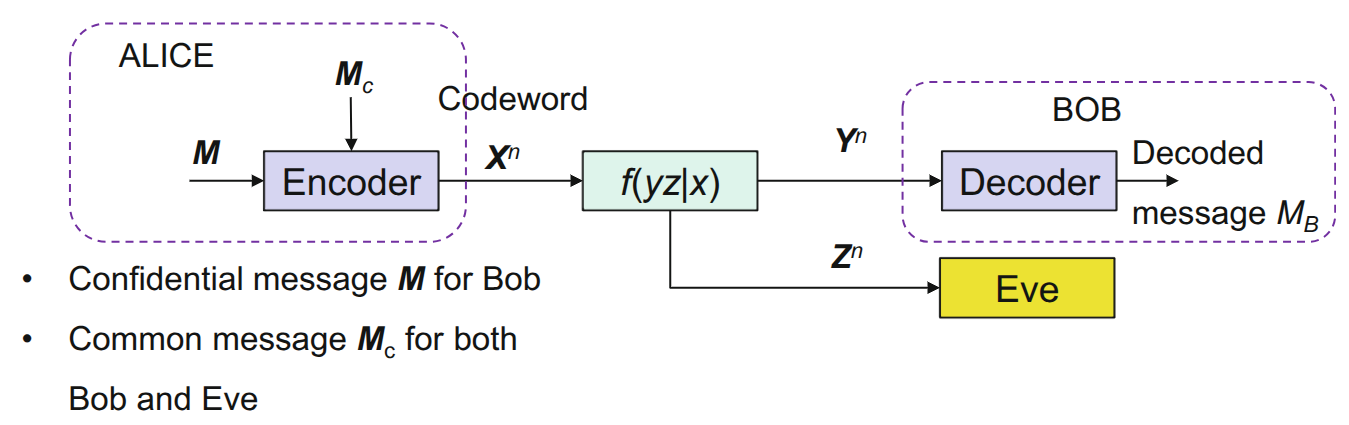
\includegraphics[width=0.8\textwidth]{chapters/figs/fig-1-5}
	\caption{مدل کانال پخش با پیام‌های محرمانه (\lr{BCC}).}
	\label{fig:1-5}
\end{figure}

یک کد شنود $(n, k)$ با نرخ $R = k/n$ توسط موارد زیر مشخص می‌شود \cite{1-3, 1-31}: (۱) مجموعه پیام‌های $M$ با اندازه $2^{nR}$، (۲) منبع تصادفی محلی $U$ با توزیع $f_U$، (۳) رمزگذاری که نگاشت پیام و یک تحقق تصادفی از منبع محلی را به یک کلمه کد انجام می‌دهد، و (۴) رمزگشایی که نگاشت کلمه دریافت‌شده به تخمین پیام را انجام می‌دهد. بزرگترین نرخ ارسالی که در آن هر دو شرط قابلیت اطمینان و محرمانگی به‌طور هم‌زمان برقرار باشند، معمولاً ظرفیت محرمانگی\LTRfootnote{Secrecy capacity} نامیده می‌شود. برای هر توزیع $f_x$ از $X$ از مجموعه‌ای از توزیع‌های $\mathcal{P}$ ($R \geq 0$) که برای آن‌ها $I(X, Y) \geq R$ است، واینر تابعی را تعریف کرده است که می‌توان آن را نرخ محرمانگی\LTRfootnote{Secrecy rate} نامید:

\begin{equation}
	SR(R) = \sup_{f_x \in \mathcal{P}(R)} [ I(X; Y) - I(X; Z) ].
	\label{eq:1-7}
\end{equation}
او همچنین نشان داد که نرخ محرمانگی\LTRfootnote{Secrecy rate} $SR(R)$ از بالا توسط ظرفیت کانال اصلی $C_m$ و از پایین توسط $C_m - C_e$ محدود می‌شود، که در آن $C_e$ ظرفیت آبشار کانال شنود اصلی است، یعنی:
\begin{equation}
	C_m - C_e \leq SR(R) \leq C_m.
	\label{eq:1-8}
\end{equation}
کانال شنود واینر توسط سیزار و کورنر تعمیم و بهبود یافت \cite{1-32} و مدل متناظر آن، که اکنون با نام کانال پخش با پیام‌های محرمانه (\lr{BCC})\LTRfootnote{Broadcast channel with confidential messages (BCC)} شناخته می‌شود، در شکل \ref{fig:1-5} ارائه شده است. فرض می‌شود که کانال پخش، گسسته و بدون حافظه\LTRfootnote{Discrete memoryless} باشد و توسط الفبای ورودی $\mathcal{X}$، الفباهای خروجی $\mathcal{Y}$ و $\mathcal{Z}$ (به‌ ترتیب مربوط به باب و ایو) و \lr{PDF} انتقال $f(yz|x)$ مشخص گردد. بنابراین، خودِ کانال توسط یک \lr{PDF} مشترک برای مشاهدات باب و ایو، $f(yz|x)$، به شرط ورودی کانال مدل‌سازی می‌شود. در این سناریو، آلیس مایل است یک پیام عمومی $M_c$ را برای هر دو گیرنده باب و ایو، و یک پیام محرمانه $M$ را برای باب پخش کند. کد تصادفی متناظر $\mathcal{C}_n$ با طول کلمه کد $n$ از موارد زیر تشکیل شده است:

\begin{itemize}
	\item دو مجموعه پیام: مجموعه پیام‌های عمومی و مجموعه پیام محرمانه.
	\item تابع رمزگذاری (تصادفی) که جفت پیام محرمانه-عمومی را به یک کلمه کد نگاشت می‌کند.
	\item دو تابع رمزگشایی: اولی که بردار مشاهده $\bm{y}^n$ را به جفت پیام تخمینی نگاشت می‌کند، در حالی که دومی بردار مشاهده $\bm{z}^n$ را به تخمین پیام عمومی نگاشت می‌نماید.
\end{itemize}

سیزار و کورنر نتیجه‌ای را اثبات کردند \cite{1-32} که بر اساس آن ظرفیت محرمانگی\LTRfootnote{Secrecy capacity} زمانی که نرخ پیام عمومی صفر تنظیم شود، به‌صورت تفاضل اطلاعات متقابل برای پیوندهای آلیس-باب و آلیس-ایو تعیین می‌شود، یعنی:
\begin{equation}
	C_s = \max_{\stackrel{f_{VX}}{V \to X \to YZ}} [ I(V; Y) - I(V; Z) ],
	\label{eq:1-9}
\end{equation}
که در آن بیشینه‌سازی روی تمام توزیع‌های مشترک ممکن $f_{VX}(v, x)$ انجام می‌شود و $V$، $X$ و $YZ$ یک زنجیره مارکوف $V \to X \to YZ$ را تشکیل می‌دهند. به‌وضوح، ظرفیت محرمانگی زمانی که کانال باب نویز کمتری نسبت به کانال ایو داشته باشد، یعنی $I(X; Y) > I(X; Z)$، اکیداً مثبت است. به‌ویژه، با قرار دادن $V = X$، عبارت ظرفیت محرمانگی به‌صورت $C_s = \max_{f_X} [ I(X; Y) - I(X; Z) ]$ در می‌آید که در صورت برقرار بودن $I(X; Y) > I(X; Z)$، اکیداً مثبت خواهد بود.
در مقایسه با رویکردهای رمزنگاری متداول که در آن‌ها از طرح‌های کدگذاری کنترل خطا (\lr{ECC})\LTRfootnote{Error control coding (ECC)} قوی برای فراهم‌سازی ارتباطات قابل‌اطمینان استفاده می‌شود، ارسال در سناریوی امنیت لایه فیزیکی (\lr{PLS}) باید به‌طور هم‌زمان قابل‌اطمینان و امن باشد. این امر نشان می‌دهد که باید کلاس‌های متفاوتی از کدهای کانال توسعه یابند. متناوباً، مشابه با \lr{QKD}، می‌توان از تصادفی بودن کانال برای تولید کلید بهره‌برداری کرد و این رویکرد معمولاً با عنوان توافق کلید مخفی\LTRfootnote{Secret-key agreement} شناخته می‌شود؛ این مفهوم در شکل \ref{fig:1-6} با الهام از مراجع \cite{1-2, 1-3, 1-6} توصیف شده است. آلیس و باب ظرفیت کانال آلیس-باب (که با نام ظرفیت کانال اصلی نیز شناخته می‌شود) $C_M$ و ظرفیت محرمانگی\LTRfootnote{Secrecy capacity} $C_S$ را که به‌صورت تفاضل بین ظرفیت کانال اصلی و ظرفیت کانال شنود $C_E$ تعریف می‌شود، پایش می‌کنند. زمانی که ظرفیت محرمانگی به‌خوبی بالاتر از مقدار آستانه $C_{S,tsh}$ و ظرفیت کانال اصلی به‌خوبی بالاتر از مقدار آستانه $C_{M,tsh}$ باشد، آلیس نمادهای با شکل گاوسی $X$ را برای باب ارسال می‌کند. هنگامی که هر دو ظرفیت محرمانگی و ظرفیت کانال اصلی به دلیل محوشدگی عمیق\LTRfootnote{Deep fading} در کانال‌های بی‌سیم یا اثرات تلاطم اتمسفری\LTRfootnote{Atmospheric turbulence} در کانال‌های نوری فضای آزاد پایین‌تر از آستانه‌های مربوطه قرار می‌گیرند، آلیس و باب مصالحه اطلاعات\LTRfootnote{Information reconciliation} نمادهای ارسال‌شده قبلی را انجام می‌دهند که بر پایه یک طرح \lr{ECC} قوی است تا اطمینان حاصل شود خطاهای وارد شده توسط کانال یا ایو قابل اصلاح هستند. مشابه طرح‌های \lr{QKD} \cite{1-7, 1-8, 1-9, 1-10, 1-11}، می‌توان از یک کد بررسی توازن کم‌چگال (\lr{LDPC})\LTRfootnote{Low-density parity-check (LDPC)} سیستماتیک استفاده کرد (که بر بیت‌های اطلاعات تأثیری نمی‌گذارد اما بیت‌های توازن\LTRfootnote{Parity bits} مرتبط جبری با بیت‌های اطلاعات را تولید می‌کند) تا بیت‌های توازن تولید شده و از طریق یک کانال عمومی احرازهویت‌شده\LTRfootnote{Authenticated public channel} ارسال گردند. طرح‌های مصالحه اطلاعات مستقیم و معکوس وجود دارند. در مصالحه مستقیم که در شکل \ref{fig:1-6} نشان داده شده است، آلیس رمزگذاری \lr{LDPC} را انجام داده و بیت‌های توازن را برای باب می‌فرستد. باب رمزگشایی \lr{LDPC} را برای به‌دست آوردن کلید صحیح $X$ انجام می‌دهد. در مصالحه معکوس، باب به جای آلیس رمزگذاری \lr{LDPC} را انجام می‌دهد. سپس تقویت حریم خصوصی\LTRfootnote{Privacy amplification} بین آلیس و باب انجام می‌شود تا از $X$ مجموعه کوچک‌تری از بیت‌های $K$ (کلید نهایی) استخراج گردد که همبستگی آن با رشته ایو پایین‌تر از یک آستانه مطلوب باشد \cite{1-9, 1-10, 1-11, 1-33}. یکی از راه‌های انجام تقویت حریم خصوصی، استفاده از توابع هش سراسری\LTRfootnote{Universal hash functions} $G$ است \cite{1-9, 1-10, 1-11, 1-33}، که مجموعه رشته‌های $n$-بیتی $X$ را به مجموعه رشته‌های $m$-بیتی $K$ نگاشت می‌کنند، به‌طوری که برای هر دو رشته متمایز $X_1$ و $X_2$ از مجموعه کلیدهای اصلاح‌شده، زمانی که نگاشت $g$ به‌صورت یکنواخت و تصادفی از $G$ انتخاب شود، احتمال برقراری $g(X_1) = g(X_2)$ بسیار پایین باشد. به‌طور معمول دو نوع مدل برای توافق کلید مخفی در نظر گرفته می‌شود \cite{1-34}:

\begin{itemize}
	\item \textbf{مدل نوع منبع\LTRfootnote{Source-type model}:} که در آن ترمینال‌ها خروجی همبسته منبع تصادفی را بدون داشتن کنترل بر آن مشاهده می‌کنند.
	\item \textbf{مدل نوع کانال\LTRfootnote{Channel-type model}:} که در آن یک ترمینال نمادهای تصادفی را با استفاده از یک کانال پخش برای ترمینال‌های دیگر ارسال می‌کند. این سناریو مشابه مدل کانال شنود با کانال بازخورد است که یک کانال عمومی احرازهویت‌شده بدون نویز محسوب می‌شود.
\end{itemize}

هر دوی این مدل‌ها بسیار شبیه به \lr{QKD} هستند \cite{1-7, 1-8, 1-9, 1-10, 1-11, 1-35, 1-36, 1-37, 1-38}، با این تفاوت که کلید خام در \lr{PLS} از طریق کانال کلاسیک ارسال می‌شود، در حالی که در \lr{QKD} از طریق کانال کوانتومی ارسال می‌گردد. پروتکل‌های توافق کلید مخفی علاوه بر شرط قابلیت اطمینان و شرط محرمانگی، باید شرط یکنواختی\LTRfootnote{Uniformity condition} را نیز ارضا کنند، که تضمین می‌کند کلید مخفی به‌طور یکنواخت در مجموعه مربوطه توزیع شده است. نرخی که کلید مخفی در آن تولید می‌شود را می‌توان مشابه \lr{QKD}، نرخ کلید مخفی (\lr{SKR})\LTRfootnote{Secret-key rate (SKR)} نامید. اگر پروتکل‌ها از پیام‌های عمومی ارسالی تنها در یک جهت (یا از آلیس به باب و یا از باب به آلیس) بهره‌برداری کنند، گفته می‌شود \lr{SKR} متناظر با ارتباط یک‌طرفه\LTRfootnote{One-way communication} دستیابی‌پذیر است؛ در غیر این صورت، گفته می‌شود \lr{SKR} با ارتباط دوطرفه\LTRfootnote{Two-way communication} دستیابی‌پذیر است. ما می‌گوییم نرخ کلید مخفی $R$ دستیابی‌پذیر است اگر دنباله‌ای از پروتکل‌های تولید کلید مخفی وجود داشته باشد که هر سه شرط (محدودیت) را در حالت $n \to \infty$ ارضا کند. سوپریمم نرخ‌های \lr{SKR} دستیابی‌پذیر معمولاً ظرفیت کلید مخفی\LTRfootnote{Secret-key capacity} نامیده شده و در اینجا با $C_{SK}$ نشان داده می‌شود. با فرض ارتباط دوطرفه روی کانال عمومی احرازهویت‌شده، استخراج یک عبارت دقیق برای $C_{SK}$ دشوار است؛ با این حال، بر اساس مراجع \cite{1-34, 1-39}، می‌توان آن را به‌صورت زیر از هر دو طرف محدود کرد:
\begin{equation}
	\max_{f_X} [ \max(I(X; Y) - I(X; Z), I(Y; X) - I(Y; Z)) ] \leq C_{SK} \leq \max_{f_X} I(X; Y|Z)
	\label{eq:1-10}
\end{equation}
جمله کران بالا نشان‌دهنده ظرفیت کلید مخفی در حالتی است که باب به مشاهدات ایو دسترسی داشته باشد. جمله کران پایین $\max[I(X; Y) - I(X; Z)]$ نشان‌دهنده به‌کارگیری مصالحه مستقیم\LTRfootnote{Direct reconciliation} است، در حالی که جمله کران پایین دیگر یعنی $\max[I(Y; X) - I(Y; Z)]$ نشان می‌دهد که به جای آن از مصالحه معکوس\LTRfootnote{Reverse reconciliation} استفاده شده است.
به‌طور خلاصه، \lr{PLS} به روش‌ها و الگوریتم‌های مختلفی مربوط می‌شود که امنیت را با بهره‌برداری از ویژگی‌های محیط فیزیکی فراهم می‌کنند. جزئیات بیشتر درباره طرح‌های مختلف \lr{PLS} را می‌توان در سایر فصل‌ها یافت.

\section{مبانی توزیع کلید کوانتومی (QKD)}
\label{sec:1-2}
اخیراً دستاوردهای قابل‌توجهی در محاسبات کوانتومی حاصل شده است \cite{1-9, 1-10, 1-11}. شرکت‌های بسیاری در حال حاضر بر روی توسعه کامپیوترهای کوانتومی با مقیاس متوسط کار می‌کنند. با توجه به اینکه اکثر سیستم‌های رمزنگاری به فرض دشواری محاسباتی\LTRfootnote{Computational hardness assumption} وابسته هستند، محاسبات کوانتومی چالشی جدی برای سیستم‌های امنیت سایبری مدرن محسوب می‌شود. به‌عنوان مثال، برای شکستن پروتکل \lr{RSA} \cite{1-26}، نیاز است که دوره تناوب $r$ تابع $f(x) = m^x \pmod n = f(x+r)$ تعیین شود ($r = 0, 1, \dots, 2^l - 1$؛ و $m$ عددی صحیح و کوچک‌تر از $n-1$ است). این دوره تناوب در یکی از مراحل الگوریتم تجزیه شور تعیین می‌شود \cite{1-9, 1-10, 1-11, 1-27, 1-28, 1-29}.

توزیع کلید کوانتومی (\lr{QKD}) با رمزگذاری متقارن\LTRfootnote{Symmetric encryption} را می‌توان به‌عنوان یکی از طرح‌های امنیت لایه فیزیکی تفسیر کرد که می‌تواند امنیت اثبات‌پذیری\LTRfootnote{Provable security} را در برابر حملات آغاز شده توسط کامپیوترهای کوانتومی فراهم کند \cite{1-35}. اولین طرح \lr{QKD} توسط بنت\LTRfootnote{Bennett} و براسارد\LTRfootnote{Brassard} معرفی شد که آن را در سال ۱۹۸۴ پیشنهاد کردند \cite{1-7, 1-8} و اکنون با نام پروتکل \lr{BB84} شناخته می‌شود. امنیت \lr{QKD} توسط قوانین مکانیک کوانتومی تضمین شده است. درجات آزادی\LTRfootnote{Degrees of freedom (DOF)} مختلف فوتون مانند قطبش، زمان، فرکانس، فاز و تکانه زاویه‌ای مداری\LTRfootnote{Orbital angular momentum} را می‌توان برای پیاده‌سازی پروتکل‌های مختلف \lr{QKD} به کار گرفت. به‌طور کلی، بسته به استراتژی اعمال شده در سمت باب، دو طرح کلی \lr{QKD} وجود دارد: \lr{QKD} با متغیر گسسته\LTRfootnote{Discrete variable (DV)} (\lr{DV-QKD}) و \lr{QKD} با متغیر پیوسته\LTRfootnote{Continuous variable (CV)} (\lr{CV-QKD}). در طرح‌های \lr{DV-QKD}، یک آشکارساز تک‌فوتون\LTRfootnote{Single-photon detector (SPD)} (\lr{SPD}) در سمت باب به کار می‌رود، در حالی که در \lr{CV-QKD} مؤلفه‌های مربعی میدان\LTRfootnote{Field quadratures} با کمک آشکارسازی هموداین/هتروداین\LTRfootnote{Homodyne/heterodyne detection} اندازه‌گیری می‌شوند. طرح \lr{DV-QKD} با به‌کارگیری قضیه کپی‌ناپذیری\LTRfootnote{No-cloning theorem} و قضیه تمایزناپذیری\LTRfootnote{Indistinguishability} حالت‌های کوانتومی دلخواه به امنیت غیرمشروط دست می‌یابد. قضیه کپی‌ناپذیری بیان می‌کند که حالت‌های کوانتومی دلخواه را نمی‌توان کپی کرد، که نشان‌دهنده این است که ایو نمی‌تواند حالت‌های کوانتومی غیرمتعامد\LTRfootnote{Non-orthogonal} را حتی با کمک کامپیوتر کوانتومی تکثیر کند. از سوی دیگر، قضیه دوم بیان می‌کند که حالت‌های غیرمتعامد را نمی‌توان به‌طور ابهام‌ناپذیر متمایز کرد. به‌ویژه، هنگامی که ایو با حالت‌های کوانتومی ارسالی تعامل برقرار می‌کند تا اطلاعاتی درباره بیت‌های ارسالی به‌دست آورد، به‌طور ناخواسته وفاداری\LTRfootnote{Fidelity} حالت‌های کوانتومی را مختل می‌کند که توسط باب شناسایی خواهد شد. از طرف دیگر، \lr{CV-QKD} از اصل عدم قطعیت\LTRfootnote{Uncertainty principle} بهره می‌برد که بیان می‌کند هر دو مؤلفه هم‌فاز\LTRfootnote{In-phase} و مربعی\LTRfootnote{Quadrature} حالت‌های همدوس را نمی‌توان به‌طور هم‌زمان با دقت کامل اندازه‌گیری کرد. ما همچنین می‌توانیم طرح‌های مختلف \lr{QKD} را در دو نوع «به کمک درهم‌تنیدگی» یا «آماده‌سازی-و-اندازه‌گیری»\LTRfootnote{Prepare-and-measure} طبقه‌بندی کنیم.

پژوهش در \lr{QKD} در حال شتاب گرفتن است، به‌ویژه پس از اولین نمایش \lr{QKD} ماهواره به زمین \cite{1-36}. اخیراً \lr{QKD} در مسافت ۴۰۴ کیلومتری از فیبر نوری با تلفات بسیار کم نمایش داده شده است؛ با این حال، نرخ کلید امن بسیار پایینی ($3.2 \times 10^{-4}$ بیت بر ثانیه) داشت. با توجه به اینکه حالت‌های کوانتومی قابل تقویت نیستند، تضعیف فیبر مسافت را محدود می‌کند. از سوی دیگر، زمان مرده\LTRfootnote{Deadtime} (مدت زمانی که یک \lr{SPD} به دلیل زمان بازیابی طولانی نسبت به فوتون‌های ورودی پاسخگو نیست) در \lr{SPD}ها که معمولاً در محدوده ۱۰ تا ۱۰۰ نانوثانیه است، نرخ باود\LTRfootnote{Baud rate} و در نتیجه نرخ کلید امن را محدود می‌کند. طرح‌های \lr{CV-QKD} از آنجا که از آشکارسازی هموداین/هتروداین استفاده می‌کنند، محدودیت زمان مرده ندارند؛ اما مسافت‌های معمول آن‌ها کوتاه‌تر است.

آلیس و باب با ارسال حالت‌های کیوبیت غیرمتعامد بین خود و بررسی اختلال در حالت ارسالی ناشی از کانال یا فعالیت ایو، می‌توانند حد بالایی برای نویز یا شنود در کانال ارتباطی کوانتومی خود تعیین کنند \cite{1-9}. آستانه حداکثر نرخ خطای تحمل‌پذیر توسط بازدهی بهترین مراحل پس‌پردازش تعیین می‌شود \cite{1-9}. پروتکل‌های \lr{QKD} را می‌توان به چندین دسته کلی تقسیم کرد:
\begin{itemize}
	\item \textbf{\lr{QKD} وابسته به دستگاه\LTRfootnote{Device-dependent QKD}:} که در آن معمولاً منبع کوانتومی در سمت آلیس و آشکارساز کوانتومی در سمت باب قرار دارد. کلاس‌های محبوب شامل \lr{DV-QKD}، \lr{CV-QKD}، \lr{QKD} به کمک درهم‌تنیدگی (\lr{EA}) و مرجع فاز توزیع‌شده\LTRfootnote{Distributed phase reference} است. برای \lr{EA-QKD}، منبع درهم‌تنیده را می‌توان در میانه کانال قرار داد تا مسافت ارسال افزایش یابد.
	\item \textbf{\lr{QKD} مستقل از دستگاه منبع:} که در آن منبع کوانتومی در سمت چارلی (ایو) قرار داده می‌شود، در حالی که آشکارسازهای کوانتومی در هر دو سمت آلیس و باب هستند.
	\item \textbf{\lr{QKD} مستقل از دستگاه اندازه‌گیری (\lr{MDI-QKD}):} که در آن آشکارسازهای کوانتومی در سمت چارلی (ایو) قرار می‌گیرند، در حالی که منابع کوانتومی در هر دو سمت آلیس و باب قرار دارند. حالت‌های کوانتومی در هر دو سمت آلیس و باب آماده‌سازی شده و به سمت آشکارسازهای چارلی ارسال می‌شوند. چارلی اندازه‌گیری‌های حالت بل\LTRfootnote{Bell state measurements} جزئی را انجام داده و زمانی که حالت بل جزئی مورد نظر شناسایی شد، آن را اعلام می‌کند؛ جزئیات بیشتر در فصل‌های بعدی ارائه خواهد شد.
\end{itemize}

\lr{QKD} می‌تواند به امنیت غیرمشروط\LTRfootnote{Unconditional security} دست یابد، به این معنی که امنیت آن را می‌توان بدون اعمال هیچ‌گونه محدودیتی بر توان محاسباتی یا استراتژی شنود ایو، تأیید کرد. کران‌های مربوط به نرخ کسر\LTRfootnote{Fraction rate} به مراحل پس‌پردازش کلاسیک\LTRfootnote{Classical postprocessing} بستگی دارد. رایج‌ترین روش، پس‌پردازش یک‌طرفه\LTRfootnote{One-way postprocessing} است که در آن آلیس یا باب کلید مرجع را در اختیار دارد و اطلاعات کلاسیک را از طریق کانال عمومی برای طرف دیگر ارسال می‌کند، در حالی که طرف مقابل بدون ارائه بازخورد، فرآیند خاصی را روی داده‌ها انجام می‌دهد. معمول‌ترین پردازش یک‌طرفه شامل دو مرحله است: مصالحه اطلاعات\LTRfootnote{Information reconciliation} و تقویت حریم خصوصی\LTRfootnote{Privacy amplification}. عبارت مربوط به کسر مخفی\LTRfootnote{Secret fraction} که از طریق پس‌پردازش یک‌طرفه به‌دست می‌آید، بسیار شبیه به طرح‌های \lr{PLS} کلاسیک است و به‌صورت زیر داده می‌شود:
\begin{equation}
	r = I(\bm{A}; \bm{B}) - \min_{\text{Eve's strategies}} (I_{EA}, I_{EB})
	\label{eq:1-11}
\end{equation}
که در آن $I(\bm{A}; \bm{B})$ اطلاعات متقابل\LTRfootnote{Mutual information} بین آلیس و باب است، در حالی که جمله دوم متناظر با اطلاعات ایو ($I_E$) درباره کلید خام آلیس یا باب است و کمینه‌سازی روی تمام استراتژی‌های شنود ممکن انجام می‌شود. آلیس و باب تصمیم خواهند گرفت که از مصالحه مستقیم یا معکوس استفاده کنند تا بتوانند اطلاعات ایو را کمینه نمایند.

اکنون استراتژی‌های مختلف شنود را که ایو ممکن است به کار گیرد و اطلاعات ایو $I_E$ را تعیین می‌کنند، شرح می‌دهیم. حملات مستقل (انفرادی) یا غیرهمدوس\LTRfootnote{Independent (individual) or incoherent attacks} محدودترین خانواده از حملات را تشکیل می‌دهند که در آن‌ها ایو به هر کیوبیت به‌طور مستقل حمله کرده و با اعمال استراتژی یکسان با هر کیوبیت تعامل می‌کند. علاوه بر این، او حالت‌های کوانتومی را پیش از انجام پس‌پردازش کلاسیک اندازه‌گیری می‌نماید. کران امنیت برای حملات غیرهمدوس مشابه کران امنیت در \lr{PLS} کلاسیک است که در آن اطلاعات متقابل بین آلیس و ایو به‌صورت زیر داده می‌شود:
\begin{equation}
	I_{EA} = \max_{\text{Eve's strategies}} I(\bm{A}; \bm{E})
	\label{eq:1-12}
\end{equation}
که در آن بیشینه‌سازی روی تمام استراتژی‌های شنود غیرهمدوس ممکن انجام می‌شود. تعریف مشابهی برای $I_{BE}$ نیز برقرار است.

حملات دسته‌جمعی\LTRfootnote{Collective attacks} نشان‌دهنده تعمیمی از حملات غیرهمدوس هستند، با این فرض که تعامل ایو با هر بیت کوانتومی (که با نام کیوبیت\LTRfootnote{Qubit} نیز شناخته می‌شود) نیز به‌صورت مستقل و با توزیع یکسان (\lr{i.i.d.})\LTRfootnote{Independent and identically distributed (i.i.d.)} است. با این حال، در این حملات ایو می‌تواند کیوبیت‌های کمکی\LTRfootnote{Ancilla qubits} خود را تا پایان مراحل پس‌پردازش کلاسیک در یک حافظه کوانتومی\LTRfootnote{Quantum memory} ذخیره کند. کران امنیت برای حملات دسته‌جمعی با فرض پس‌پردازش یک‌طرفه، توسط رابطه \eqref{eq:1-11} داده می‌شود که در آن اطلاعات ایو درباره دنباله آلیس بر اساس اطلاعات هولِوو\LTRfootnote{Holevo information} به‌صورت زیر تعیین می‌شود \cite{1-37, 1-38}:
\begin{equation}
	I_{EA} = \max_{\text{Eve's strategies}} \chi(\bm{A}; \bm{E})
	\label{eq:1-13}
\end{equation}
که در آن بیشینه‌سازی روی تمام استراتژی‌های شنود دسته‌جمعی ممکن انجام می‌شود. تعریف مشابهی نیز برای $I_{BE}$ برقرار است. این کران با نام کران دوتک-وینتر\LTRfootnote{Devetak-Winter bound} نیز شناخته می‌شود. اطلاعات هولِوو که در مرجع \cite{1-40} معرفی شده است، در اینجا به‌صورت زیر تعریف می‌گردد:
\begin{equation}
	\chi(\bm{A}; \bm{E}) = S(\rho_E) - \sum_{a} p(a) S(\rho_{E|a})
	\label{eq:1-14}
\end{equation}
که در آن $S(\rho)$ آنتروپی فون نویمان\LTRfootnote{von Neumann entropy} است که به‌صورت $S(\rho) = -\text{Tr}(\rho \log \rho) = -\sum_{i} \lambda_i \log \lambda_i$ تعریف می‌شود و در آن $\lambda_i$ مقادیر ویژه عملگر (حالت) چگالی\LTRfootnote{Density operator} $\rho$ هستند. عملگر چگالی برای بازنمایی مجموعه‌ای\LTRfootnote{Ensemble} از حالت‌های کوانتومی استفاده می‌شود که هر کدام با احتمالی معین رخ می‌دهند. (برای جزئیات بیشتر درباره عملگرهای چگالی به فصل \ref{chap:5} مراجعه کنید.) در رابطه \eqref{eq:1-14}، $p(a)$ نشان‌دهنده احتمال وقوع نماد $a$ از الفبای کلاسیک آلیس است، در حالی که $\rho_{E|a}$ عملگر چگالی متناظر با سیستم کمکی ایو است. در نهایت، $\rho_E$ حالت چگالی جزئی ایو است که به‌صورت $\rho_E = \sum_{a} p(a) \rho_{E|a}$ تعریف می‌شود. به عبارت دیگر، اطلاعات هولِوو متناظر با میانگین کاهش در آنتروپی فون نویمان است، با این فرض که می‌دانیم $\rho_E$ چگونه آماده‌سازی شده است.

\section{سازمان‌دهی کتاب}
\label{sec:1-3}
این کتاب به‌صورت زیر سازمان‌دهی شده است. در پایان هر فصل، مجموعه‌ای از مسائل برای کمک به خواننده در دستیابی به درک عمیق‌تر از مفاهیم شرح داده شده در آن فصل ارائه شده است. پس از مقدمه، در فصل \ref{chap:2}، مفاهیم نظریه اطلاعات\LTRfootnote{Information theory} کلاسیک به همراه کاربرد متناظر آن‌ها در کانال‌های محوشدگی\LTRfootnote{Fading channels} و کانال‌های دارای حافظه\LTRfootnote{Channels with memory} ارائه می‌شوند. این فصل مبانی نظریه اطلاعات و کدگذاری را در سطحی فراهم می‌کند که برای دنبال کردن آسان مطالب کتاب مورد نیاز است. فصل با تعاریف آنتروپی، آنتروپی مشترک، آنتروپی شرطی، آنتروپی نسبی\LTRfootnote{Relative entropy}، اطلاعات متقابل و ظرفیت کانال آغاز شده و با قضیه ظرفیت اطلاعات ادامه می‌یابد. ما درباره ظرفیت کانال در کانال‌های گسسته بدون حافظه، کانال‌های پیوسته و کانال‌های دارای حافظه بحث می‌کنیم. در رابطه با کانال‌های بی‌سیم، نحوه محاسبه ظرفیت کانال در کانال‌های محوشدگی هموار\LTRfootnote{Flat-fading} و گزینش‌گر فرکانس\LTRfootnote{Frequency-selective} را شرح می‌دهیم. همچنین استراتژی‌های مختلف بهینه و زیربهینه برای دستیابی به ظرفیت کانال، از جمله روش پر کردن آب\LTRfootnote{Water-filling method}، کدگذاری و رمزگشایی تسهیم‌شده، وارون‌سازی کانال و وارون‌سازی کانال کوتاه شده\LTRfootnote{Truncated channel inversion} را مورد بحث قرار می‌دهیم. علاوه بر این، استراتژی‌های مختلف برای محاسبه ظرفیت کانال بسته به آنچه از اطلاعات وضعیت کانال\LTRfootnote{Channel state information (CSI)} دانسته می‌شود، مطالعه می‌گردند. در ادامه، نحوه مدل‌سازی کانال دارای حافظه را توضیح داده و مدل مک‌میلان-خینچین\LTRfootnote{McMillan-Khinchin model} را برای ارزیابی ظرفیت کانال تشریح می‌کنیم. سپس، مبانی کدهای بلوکی خطی و به‌دنبال آن مبانی کدگذاری \lr{LDPC} باینری معرفی می‌شوند. پس از ملاحظات پایانی، مجموعه‌ای از مسائل ارائه شده است.

در فصل \ref{chap:3}، مبانی رمزنگاری متداول معرفی می‌شوند. ابتدا اصطلاحات پایه و طرح‌های رمزنگاری، شامل رمزنگاری متقارن و نامتقارن، رمزهای پایه مانند رمزهای جایگزینی\LTRfootnote{Substitution ciphers} و جابه‌جایی\LTRfootnote{Transposition ciphers}، و پد‌های یک‌بار مصرف معرفی می‌گردند. مفاهیم محرمانگی، احراز هویت و انکارناپذیری\LTRfootnote{Non-repudiation} مورد بحث قرار می‌گیرند و به‌دنبال آن حملات مختلف تحلیل رمز\LTRfootnote{Cryptanalytic attacks} مانند حملات فقط-رمزنگاشت\LTRfootnote{Ciphertext-only}، متن‌آشکار-معلوم\LTRfootnote{Known-plaintext}، متن‌آشکار-انتخابی\LTRfootnote{Chosen-plaintext}، رمزنگاشت-انتخابی\LTRfootnote{Chosen-ciphertext} و متن‌آشکار-انتخابی سازگار\LTRfootnote{Adaptive chosen-plaintext} بررسی می‌شوند. مفهوم امنیت کامل در ادامه معرفی شده و با امنیت محاسباتی مقایسه می‌گردد. در همان بخش، فاصله یکتایی\LTRfootnote{Unicity distance} و همچنین نقش فشرده‌سازی در رمزنگاری مورد بحث قرار می‌گیرد. سپس، توابع یک‌طرفه و توابع هش یک‌طرفه بررسی می‌شوند. فصل با چندین سیستم رمزنگاری کاربردی مرتبط، شامل سیستم‌های \lr{DES} و \lr{RSA} و همچنین توزیع کلید عمومی دیفی-هلمن\LTRfootnote{Diffie-Hellman} به پایان می‌رسد. در ادامه، ملاحظات پایانی و مجموعه‌ای از مسائل ارائه شده است.

فصل \ref{chap:4} به امنیت لایه فیزیکی اختصاص یافته است. فصل با بحثی درباره مسائل امنیتی آغاز شده و با معرفی امنیت نظریه-اطلاعاتی و مقایسه آن با امنیت محاسباتی ادامه می‌یابد. در همان بخش، معیارهای مختلف امنیت نظریه-اطلاعاتی، از جمله شرایط محرمانگی قوی و ضعیف معرفی می‌شوند. سپس، مدل کانال شنود واینر که با نام مدل کانال شنود تخریب‌شده نیز شناخته می‌شود، معرفی می‌گردد. در همان بخش، مفهوم ظرفیت محرمانگی و همچنین کدگذاری شنود آشیانه‌ای\LTRfootnote{Nested wiretap coding} معرفی می‌شود. علاوه بر این، کانال پخش با پیام‌های محرمانه معرفی شده و تعریف ظرفیت محرمانگی تعمیم داده می‌شود. سپس تمرکز به سمت تولید (توافق) کلید مخفی معطوف شده، مدل‌های نوع منبع و کانال معرفی می‌شوند و پروتکل‌های تولید کلید مخفی متناظر تشریح می‌گردند. بخش بعدی به کدگذاری برای سیستم‌های امنیت لایه فیزیکی، شامل کدگذاری برای سیستم‌های محرمانگی ضعیف و قوی اختصاص دارد. در رابطه با کدگذاری برای سیستم‌های محرمانگی ضعیف، توجه ویژه‌ای به کدگذاری \lr{LDPC} از نوع دو-لبه\LTRfootnote{Two-edge-type}، کدگذاری \lr{LDPC} پنچرشده\LTRfootnote{Punctured} و کدهای قطبی معطوف شده است. در مورد کدگذاری برای سیستم‌های محرمانگی قوی، تمرکز بر کدگذاری هم‌مجموعه‌ای\LTRfootnote{Coset coding} با کدهای \lr{LDPC} دوگان و کدگذاری مبتنی بر توابع هش/استخراج‌کننده\LTRfootnote{Extractor-based} است. سپس توجه به سمت مصالحه اطلاعات و تقویت حریم خصوصی معطوف می‌شود. در بخش \lr{PLS} کانال‌های بی‌سیم، موضوعات زیر پوشش داده می‌شوند: مبانی \lr{MIMO}، امنیت لایه فیزیکی در \lr{MIMO} بی‌سیم، و تولید کلید مخفی در شبکه‌های بی‌سیم. در بخش \lr{PLS} کانال‌های نوری، هر دو حوزه \lr{PLS} برای سیستم‌های مبتنی بر فیبرهای تسهیم‌سازی تقسیم فضایی\LTRfootnote{Spatial division multiplexing (SDM)} (\lr{SDM}) و سیستم‌های نوری فضای آزاد (\lr{FSO}) مورد بحث قرار می‌گیرند. ملاحظات پایانی در ادامه ارائه شده و به‌دنبال آن مجموعه‌ای از مسائل که برای درک بهتر مفاهیم شرح داده شده درج شده‌اند، می‌آید.


در فصل \ref{chap:5}، مفاهیم پایه پردازش اطلاعات کوانتومی\LTRfootnote{Quantum information processing}، نظریه اطلاعات کوانتومی و تصحیح خطای کوانتومی\LTRfootnote{Quantum error correction} برای درک بهتر سیستم‌های \lr{QKD} ارائه شده است. موضوعات زیر از حوزه پردازش اطلاعات کوانتومی پوشش داده شده‌اند: بردارهای حالت\LTRfootnote{State vectors}، عملگرها\LTRfootnote{Operators}، عملگرهای چگالی\LTRfootnote{Density operators}، اندازه‌گیری‌ها، دینامیک یک سیستم کوانتومی، اصل برهم‌نهی\LTRfootnote{Superposition principle}، موازی‌گرایی کوانتومی\LTRfootnote{Quantum parallelism}، قضیه کپی‌ناپذیری و درهم‌تنیدگی. مفاهیم زیر نیز از نظریه اطلاعات کوانتومی ارائه شده‌اند: اطلاعات هولِوو\LTRfootnote{Holevo information}، اطلاعات در دسترس\LTRfootnote{Accessible information}، کران هولِوو\LTRfootnote{Holevo bound}، آنتروپی شانون و آنتروپی فون نویمان، قضیه کدگذاری کوانتومی بدون نویز شوماخر\LTRfootnote{Schumacher’s noiseless quantum coding theorem} و قضیه هولِوو-شوماخر-وستمورلند\LTRfootnote{Holevo-Schumacher-Westmoreland theorem}. مفاهیم پایه تصحیح خطای کوانتومی نیز معرفی شده‌اند. در ادامه، فصل با مجموعه‌ای از مسائل به پایان می‌رسد.

فصل \ref{chap:6} به مبانی اپتیک کوانتومی و سیستم‌های متغیر پیوسته (\lr{CV}) اختصاص یافته است. ابتدا امواج الکترومغناطیسی، پتانسیل برداری و معادله موج معرفی شده و به‌دنبال آن، کوانتیزه کردن میدان‌های الکترومغناطیسی ارائه می‌شود. پس از معرفی عملگرهای مربعی\LTRfootnote{Quadrature operators}، حالت‌های فوک\LTRfootnote{Fock states}، همدوس\LTRfootnote{Coherent states} و فشرده\LTRfootnote{Squeezed states} را معرفی می‌کنیم. در ادامه، تقسیم‌کننده پرتو با استفاده از مفاهیم مکانیک کوانتومی توصیف شده و برای ساخت آشکارساز متعادل هموداین\LTRfootnote{Homodyne balanced detector} به کار می‌رود. در بخش بعدی، تداخل‌سنج ماخ-زندر کوانتومی معرفی می‌گردد. سپس، حالت‌های تابش گرمایی تشریح می‌شوند. فصل با معرفی مبانی نظریه اطلاعات کوانتومی گاوسی ادامه می‌یابد که در آن نمایش-$P$\LTRfootnote{P-representation} معرفی شده و برای نمایش نویز گرمایی و همچنین سیگنال حالت همدوس به‌همراه نویز گرمایی به کار می‌رود. علاوه بر این، حالت‌های گاوسی معرفی شده و به‌دنبال آن تعریف تابع ویگنر و ماتریس‌های همبستگی\LTRfootnote{Correlation matrices} ارائه می‌شود. زیربخش بعدی به تبدیل‌های گاوسی و کانال‌های گاوسی اختصاص دارد که عملگر تقسیم‌کننده پرتو، عملگر چرخش فاز و عملگرهای فشردگی به‌عنوان نمونه‌های شاخص آن‌ها بررسی می‌شوند. تجزیه گرمایی حالت‌های گاوسی موضوع بعدی است و آنتروپی فون نویمان برای حالت‌های گرمایی استخراج می‌شود. سپس تمرکز به سمت مبانی اپتیک کوانتومی غیرخطی معطوف شده و به‌ویژه اختلاط سه‌موج و اختلاط چهارموج به‌تفصیل شرح داده می‌شوند. در ادامه، تولید حالت‌های گاوسی توصیف شده و تولید حالت فشرده دو-مُدی\LTRfootnote{Two-mode squeeze state} به‌طور کامل مورد بحث قرار می‌گیرد. ماتریس‌های همبستگی برای حالت‌های گاوسی دو-مُدی و نحوه محاسبه مقادیر ویژه سیمپلکتیک\LTRfootnote{Symplectic eigenvalues} (مرتبط با محاسبه آنتروپی فون نویمان) در ادامه بررسی می‌شوند. اندازه‌گیری و آشکارسازی حالت‌های گاوسی با تأکید بر آشکارسازی هموداین، آشکارسازی هتروداین و اندازه‌گیری‌های جزئی مورد بحث قرار می‌گیرند. سپس ماتریس‌های کوواریانس برای حالت‌های گاوسی چندمُدی معرفی می‌شوند. در نهایت، ملاحظات پایانی و مجموعه‌ای از مسائل ارائه شده است.

فصل \ref{chap:7} به مبانی \lr{QKD} اختصاص دارد. فصل با توصیف تفاوت‌های کلیدی بین رمزنگاری متداول، \lr{PLS} کلاسیک و \lr{QKD} آغاز می‌شود. در بخش مبانی \lr{QKD}، پس از یک مرور تاریخی، انواع مختلف \lr{QKD} را مرور کرده و به‌اختصار مراحل معمول پس‌پردازش، یعنی مراحل مصالحه اطلاعات و تقویت حریم خصوصی را شرح می‌دهیم. در همان بخش، دو قضیه بنیادی که \lr{QKD} بر آن‌ها استوار است را ارائه می‌دهیم: قضیه کپی‌ناپذیری و قضیه عدم توانایی در تمایز ابهام‌ناپذیر حالت‌های کوانتومی غیرمتعامد. در بخش سیستم‌های \lr{QKD} با متغیر گسسته (\lr{DV})، پروتکل‌های \lr{BB84} و \lr{B92} و همچنین پروتکل‌های اکرت (\lr{E91}) و \lr{EPR} را به‌تفصیل توصیف می‌کنیم. در همان بخش، پروتکل کدگذاری فاز-زمان نیز شرح داده شده است. در رابطه با پروتکل‌های \lr{BB84}، نسخه‌های مختلف مناسب برای فناوری‌های گوناگون بررسی می‌شوند. در بخش امنیت \lr{QKD}، نرخ کلید مخفی به‌صورت حاصل‌ضرب نرخ کلید خام و نرخ کسری نمایش داده شده و به‌دنبال آن محدودیت‌های مختلف نرخ کلید خام توصیف می‌شوند. سپس، عبارت عمومی برای نرخ کسری ارائه شده و انواع استراتژی‌های شنود، شامل حملات انفرادی (مستقل یا غیرهمدوس)، حملات دسته‌جمعی و حملات همدوس\LTRfootnote{Coherent attacks}، و همچنین حملات هک کوانتومی/کانال جانبی تشریح می‌گردند. برای حملات انفرادی و همدوس، عبارات کسر مخفی متناظر شرح داده شده‌اند. بخش بعدی به تعاریف مختلف امنیت، از جمله مفهوم $\epsilon$-امنیت\LTRfootnote{$\epsilon$-security} اختصاص یافته است. سپس، عبارات عمومی برای طرح‌های \lr{DV-QKD} دوبعدی برای هر دو پروتکل آماده‌سازی-و-اندازه‌گیری و پروتکل‌های مبتنی بر حالت فریب استخراج می‌شوند. برای تسهیل توصیف پروتکل‌های \lr{QKD} با متغیر پیوسته (\lr{CV})، ابتدا مبانی اپتیک کوانتومی معرفی می‌شوند. در بخش پروتکل‌های \lr{CV-QKD}، هر دو نوع پروتکل مبتنی بر حالت‌های فشرده و حالت‌های همدوس تشریح می‌شوند. با توجه به اینکه تولید و دست‌کاری حالت‌های همدوس بسیار ساده‌تر است، پروتکل‌های مبتنی بر حالت همدوس با هر دو نوع آشکارسازی هموداین و هتروداین به‌تفصیل شرح داده شده‌اند. کسر مخفی برای هر دو پروتکل \lr{CV-QKD} مبتنی بر مصالحه مستقیم و معکوس استخراج شده است. علاوه‌ بر این، جزئیات جنبه‌های کاربردی پروتکل \lr{GG02} ارائه شده و محاسبه کسر مخفی برای حملات دسته‌جمعی مورد بحث قرار گرفته است. سپس، مفاهیم پایه پروتکل‌های \lr{QKD} مستقل از دستگاه اندازه‌گیری (\lr{MDI}) معرفی می‌شوند. در پایان فصل، ملاحظات پایانی و مجموعه‌ای از مسائل ارائه شده است.

فصل \ref{chap:8} در ادامه فصل \ref{chap:7} بوده و به پروتکل‌های \lr{QKD} با متغیر گسسته (\lr{DV}) اختصاص یافته است. فصل با توصیف پروتکل‌های \lr{BB84} و مبتنی بر حالت فریب، و ارزیابی عملکرد کسر محرمانگی آن‌ها برحسب مسافت دستیابی‌پذیر آغاز می‌شود. موضوع بعدی مربوط به امنیت پروتکل‌های \lr{DV-QKD} در شرایطی است که منابع محدود\LTRfootnote{Finite resources} هستند. ما مفهوم $\epsilon$-امنیت ترکیب‌پذیر\LTRfootnote{Composable $\epsilon$-security} را معرفی کرده و نحوه ارزیابی آن را برای هر دو نوع حمله دسته‌جمعی و همدوس شرح می‌دهیم. همچنین بحث می‌کنیم که چگونه مفاهیم صحت\LTRfootnote{Correctness} و محرمانگی را می‌توان برای دستیابی به کران‌های امنیتی محکم ترکیب کرد. سپس، پروتکل‌های \lr{BB84} و حالت فریب را برای فرض کلید محدود تحت اثرات تلاطم اتمسفری ارزیابی می‌کنیم. همچنین نحوه مواجهه با شرایط متغیر زمانی در کانال‌های نوری فضای آزاد توصیف می‌شود. سپس تمرکز به سمت پروتکل‌های \lr{QKD} با ابعاد بالا\LTRfootnote{High-dimensional (HD) QKD} معطوف شده و با توصیف انتخاب پایه‌های متقابلاً بدون سوگیری\LTRfootnote{Mutually unbiased bases (MUBs)} (\lr{MUBs}) و به‌دنبال آن معرفی حالت‌های بل تعمیم‌یافته آغاز می‌شود. سپس نحوه ارزیابی امنیت پروتکل‌های \lr{QKD} ابعاد بالا برای منابع محدود را شرح می‌دهیم. انواع پروتکل‌های \lr{QKD} ابعاد بالا، شامل کدگذاری فاز-زمان، کدگذاری زمان-انرژی، \lr{QKD} ابعاد بالا مبتنی بر \lr{OAM}، \lr{QKD} ابعاد بالا مبتنی بر توری‌های براگ فیبری\LTRfootnote{Fiber Bragg grating (FBGs)} (\lr{FBG}) و پروتکل‌های مبتنی بر توری‌های براگ موجبری\LTRfootnote{Waveguide Bragg gratings (WBGs)} (\lr{WBG}) توصیف می‌شوند. پس از ملاحظات پایانی، مجموعه‌ای از مسائل ارائه شده است.

فصل \ref{chap:9} به شرح تفصیلی طرح‌های \lr{CV-QKD}، به‌ویژه با مدولاسیون گاوسی و مدولاسیون گسسته اختصاص یافته است. به خواننده‌ای که با مبانی اپتیک کوانتومی و اصول سیستم‌های متغیر پیوسته (\lr{CV}) آشنا نیست، توصیه می‌شود ابتدا فصل \ref{chap:6} را مطالعه کند. در بخش مربوط به پروتکل‌های \lr{CV-QKD} با مدولاسیون گاوسی، پس از شرح کوتاهی از پروتکل‌های مبتنی بر حالت‌های فشرده، پروتکل‌های مبتنی بر حالت‌های همدوس با جزئیات کامل تشریح می‌شوند. ما این بخش را با توصیف هر دو نوع کانال ارسال بدون تلفات و با تلفات آغاز می‌کنیم. سپس هم‌ارزی بین پروتکل‌های آماده‌سازی-و-اندازه‌گیری\LTRfootnote{Prepare-and-measure (PM)} (\lr{PM}) و پروتکل‌های به کمک درهم‌تنیدگی\LTRfootnote{Entanglement-assisted} با مدولاسیون گاوسی مورد بحث قرار می‌گیرد. در ادامه، تمرکز به سمت محاسبه نرخ کلید مخفی تحت حملات دسته‌جمعی معطوف می‌شود. ابتدا محاسبه اطلاعات متقابل بین آلیس و باب بررسی شده و به‌دنبال آن محاسبه اطلاعات هولِوو بین ایو و باب، در هر دو مورد با فرض پروتکل \lr{PM} و مصالحه معکوس، انجام می‌شود. علاوه‌ بر این، حمله کپی‌کننده درهم‌تننده\LTRfootnote{Entangling-cloner attack} توصیف شده و استخراج اطلاعات هولِوو ایو-باب ارائه می‌گردد. سپس پروتکل به کمک درهم‌تنیدگی و استخراج اطلاعات هولِوو متناظر با آن تشریح می‌شود. در تمامی این استخراج‌ها، هر دو نوع آشکارسازی هموداین و هتروداین در نظر گرفته شده‌اند. همچنین برخی نتایج توصیفی \lr{SKR} مربوط به مدولاسیون گاوسی ارائه شده است. در بخش مربوط به \lr{CV-QKD} با مدولاسیون گسسته، پس از یک مقدمه کوتاه، پروتکل‌های \lr{CV-QKD} چهار-حالتی و هشت-حالتی را توصیف می‌کنیم. هر دو نوع پروتکل \lr{PM} و به کمک درهم‌تنیدگی مورد بحث قرار می‌گیرند. در ادامه، محاسبه \lr{SKR} برای مدولاسیون گسسته همراه با نتایج عددی توصیفی بررسی می‌شود. ما همچنین شرایطی را که در آن مدولاسیون گسسته می‌تواند عملکرد بهتری نسبت به مدولاسیون گاوسی داشته باشد، شناسایی می‌کنیم. در بخش طرح \lr{CV-QKD} به کمک \lr{RF}\LTRfootnote{RF-assisted}، یک طرح کلی به کمک \lr{RF} را توصیف می‌کنیم که برای طرح‌های مدولاسیون دوبعدی دلخواه، از جمله \lr{M-ary PSK} و \lr{M-ary QAM}، قابل اعمال است. این طرح در مقایسه با پروتکل‌های \lr{CV-QKD} متداول با مدولاسیون گسسته، تاب‌آوری بهتری نسبت به نویز فاز لیزر و نوسانات آفست فرکانسی نشان می‌دهد. سپس نحوه افزایش \lr{SKR} از طریق رویکرد موازی‌سازی\LTRfootnote{Parallelization} را مورد بحث قرار می‌دهیم. بخش نهایی فصل ملاحظات پایانی مرتبط را ارائه داده و به‌دنبال آن مسائل فصل می‌آیند.

فصل \ref{chap:10} به طرح‌های \lr{QKD} با متغیر گسسته (\lr{DV}) و متغیر پیوسته (\lr{CV}) که اخیراً پیشنهاد شده‌اند، اختصاص دارد. فصل با توصیف اثر هونگ-او-ماندل و اندازه‌گیری‌های حالت بل\LTRfootnote{Bell state measurements (BSMs)} (\lr{BSM}) فوتونی آغاز می‌شود. هر دو نوع \lr{BSM} مبتنی بر حالت‌های قطبش و حالت‌های بازه-زمانی\LTRfootnote{Time-bin} معرفی می‌شوند. سپس پروتکل‌های \lr{BB84} و حالت فریب به‌طور مختصر بازبینی می‌شوند. موضوع بعدی در این فصل به پروتکل‌های \lr{QKD} مستقل از دستگاه اندازه‌گیری (\lr{MDI}) اختصاص یافته است. هر دو پروتکل \lr{MDI-QKD} مبتنی بر حالت‌های قطبش و حالت‌های فاز-زمان تشریح می‌شوند. علاوه‌ بر این، پروتکل‌های \lr{QKD} میدان-دوقلو\LTRfootnote{Twin-field (TF)-QKD} (\lr{TF}) توصیف می‌شوند که قادر به شکستن کران پیراندولا-لورنزا-اوتاویانی-بانکی (\lr{PLOB}) روی نرخ کلید خطی هستند. سپس پروتکل \lr{CV-QKD} نورافکن\LTRfootnote{Floodlight (FL)} (\lr{FL}) توصیف می‌شود که قادر به دستیابی به نرخ‌های کلید مخفی رکوردشکن است. در ادامه، طرح \lr{CV-QKD} مبتنی بر گیرنده کرامرز-کرونیگ\LTRfootnote{Kramers-Kronig (KK)-receiver} (\lr{KK}) معرفی می‌گردد که نشان‌دهنده طرحی با \lr{SKR} بالا و پیچیدگی کم است. سپس طرح \lr{CV-QKD}ای تشریح می‌شود که در آن مصالحه اطلاعات از طریق یک پیوند به کمک درهم‌تنیدگی انجام می‌گیرد. در نهایت ملاحظات پایانی ارائه شده و مجموعه‌ای از مسائل برای کمک به خوانندگان در جهت کسب درک عمیق‌تر آورده شده است.

فصل \ref{chap:11} به مخابرات پنهان\LTRfootnote{Covert communications} که با نام احتمال پایین آشکارسازی/شنود\LTRfootnote{Low probability of detection/intercept} نیز شناخته می‌شود، و همچنین مخابرات رادارگریز\LTRfootnote{Stealth communications} اختصاص یافته است و اینکه چگونه این روش‌ها می‌توانند نرخ کلید مخفی را برای کاربردهای \lr{QKD} بهبود بخشند. فصل با مقدمه‌ای کوتاه بر مخابرات پنهان آغاز شده و با توصیف تفاوت‌های آن‌ها نسبت به پنهان‌نگاری\LTRfootnote{Steganography} ادامه می‌یابد. یکی از فناوری‌های کلیدی برای توانمندسازی مخابرات پنهان در کانال‌های بی‌سیم، یعنی مفهوم طیف گسترده\LTRfootnote{Spread spectrum}، در ادامه معرفی می‌شود. سپس، بررسی دقیق مخابرات پنهان در یک کانال نویز گاوسی سفید جمع‌شونده (\lr{AWGN}) ارائه شده و قانون ریشه دوم\LTRfootnote{Square root law} استخراج می‌گردد. اهمیت آزمون فرض\LTRfootnote{Hypothesis testing} در مخابرات پنهان نیز مورد بحث قرار می‌گیرد. سپس مخابرات پنهان در کانال‌های گسسته بدون حافظه بررسی می‌شود. موضوع بعدی به رویکردهای مختلف برای غلبه بر قانون ریشه دوم مربوط است، از جمله استفاده از مسدودکننده (جمر) دوست\LTRfootnote{Friendly jammer} که توان نویز را تغییر می‌دهد تا بتوان بر قانون ریشه دوم غلبه کرد و به نرخ پنهان مثبت دست یافت. مفهوم محرمانگی مؤثر\LTRfootnote{Effective secrecy} در ادامه معرفی می‌شود که یک معیار محرمانگی جدید است و تعریف آن شامل هر دو شرط محرمانگی قوی و مخابرات رادارگریز می‌باشد. سپس، مفهوم مخابرات پنهان/رادارگریز در سیستم‌های مخابرات نوری به کار گرفته می‌شود. ما در ادامه توصیف می‌کنیم که چگونه مفهوم پنهان‌سازی می‌تواند در مرحله مصالحه اطلاعات در \lr{QKD} اعمال شود تا به‌طور هم‌زمان نرخ کلید مخفی بهبود یافته و مسافت ارسال افزایش یابد. سپس نتایج تجربی مربوط به احتمال پایین شنود و مخابرات پنهان که در کانال‌های با تلاطم اتمسفری قوی عمل می‌کنند، ارائه می‌شود. بخش پایانی فصل را خلاصه کرده و مجموعه‌ای از مسائل در انتهای آن قرار گرفته است.

فصل \ref{chap:12} به مفاهیم رمزنگاری پسا‌کوانتومی\LTRfootnote{Post-quantum cryptography (PQC)} (\lr{PQC}) مربوط می‌شود. پس از مقدمه‌ای کوتاه، مفاهیم رمزنگاری مبتنی بر مشبکه\LTRfootnote{Lattice-based cryptography} زیر تشریح می‌شوند: رمزنگاری مبتنی بر یادگیری با خطا\LTRfootnote{Learning with errors (LWE)} (\lr{LWE}) ماتی\LTRfootnote{Module}، رمزنگاری مبتنی بر \lr{LWE} حلقوی، امضاهای دیجیتال مبتنی بر مشبکه و توابع هش مبتنی بر مشبکه. علاوه‌ بر این، مفاهیم رمزنگاری مبتنی بر کد\LTRfootnote{Code-based cryptography} با تمرکز بر طرح رمزگذاری مک‌الیس\LTRfootnote{McEliece}، سیستم رمزنگاری نیدرایتر\LTRfootnote{Niederreiter} و رمزگذاری مبتنی بر کدگذاری \lr{QC-LDPC} شبه‌دوری تشریح می‌شوند. در بخش بعدی، مفاهیم ترکیبی \lr{QKD-PQC} توصیف می‌شوند که در آن‌ها \lr{QKD} و \lr{PQC} به‌صورت تعاملی عمل می‌کنند. موضوع بعدی مربوط به رمزنگاری مبتنی بر هش\LTRfootnote{Hash-based cryptography} است؛ این بخش با مفاهیم پایه رمزنگاری مبتنی بر هش شامل طرح امضای یک‌بار مصرف لمپورت\LTRfootnote{Lamport} آغاز می‌شود. دو طرح رمزنگاری مبتنی بر هش مرتبط تشریح می‌شوند: طرح امضای یک‌بار مصرف وینترنیتز\LTRfootnote{Winternitz} (\lr{W-OTS}) و طرح امضای مرکل\LTRfootnote{Merkle} (\lr{MMS}) که برای امضاهای چندبار مصرف قابل اعمال است. برخی مفاهیم مرتبط با رمزنگاری چندمتغیره\LTRfootnote{Multivariate cryptography} در ادامه توصیف می‌شوند. پس از ملاحظات پایانی، مجموعه‌ای از مسائل ارائه شده است.

در پیوست، برخی مطالب پیش‌زمینه مانند مبانی جبر مجرد\LTRfootnote{Abstract algebra fundamentals} ارائه شده است که به خوانندگان ناآشنا کمک می‌کند مفاهیم امنیت لایه فیزیکی، \lr{QKD} و \lr{PQC} را بهتر درک کنند.